\documentclass[12pt]{extarticle}
%Some packages I commonly use.
\usepackage[english]{babel}
\usepackage{graphicx}
\usepackage{framed}
\usepackage[normalem]{ulem}
\usepackage{amsmath}
\usepackage{amsthm}
\usepackage{amssymb}
\usepackage{amsfonts}
\usepackage{enumerate}
\usepackage[utf8]{inputenc}
\usepackage[top=1 in,bottom=1in, left=1 in, right=1 in]{geometry}


\title{Target Illumination by GWAS Analytics (TIGA) Formulae: Gene-Trait Association Scoring}
\author{Jeremy Yang, Cristian Bologa, Stephen Mathias, Christophe Lambert, \\
David Wild, Lars Juhl Jensen  and Tudor Oprea}
\date{October 2019}

\begin{document}

\maketitle

\section{RCRAS =  Relative Citation Ratio (RCR) Aggregated Score}

The purpose is to evaluate the evidence for a gene-trait association, by aggregating multiple studies and their corresponding publications. The iCite\footnote{https://icite.od.nih.gov/} RCR\cite{rcr} is itself a statistic designed to evaluate the evolving empirical impact of a publication (in contrast to the non-empirical impact factor). Hence by aggregating RCRs we seek an corresponding measure of scientific community impact.
 
\begin{equation} RCRAS_{gt} = \sum_{study} \left(\frac{1}{gc} \sum_{pub} \frac{log_{2}(RCR + 1)}{sc}\right)
\end{equation}

Where \\
\begin{center}
\begin{tabular}{ r c l }
    $study$ & $=$ & GWAS (study\_accession) \\
	$gc$ & $=$ & gene count (in study)	\\
	$pub$ & $=$ & publication (PubMed ID)	\\
	$sc$ & $=$ & study count (in pub)	\\
\end{tabular}
\end{center}

RCR $median = 2.0$ and $90\%ile = 8.5$. The $log_{2}()$ function is used with the belief that additional publications add diminishing evidence. Division by $spp$ effects a partial count for papers associated with multiple studies. Since $RCR >= 0$, $log_{2}(RCR + 1) >= 0$ and intuitively, when $RCR = 1$ and $sc = 1$, $log_{2}(RCR + 1) = 1$,  Similarly division by $gc$ reflects a partial count since papers and studies may associate to few or many findings and reported genes. \\
\\
From NHGRI-EBI GWAS Catalog\footnote{https://www.ebi.ac.uk/gwas/} and iCite PubMed statistics. \\
\\
This approach informed by bibliometric methodology, including fractional counting, of Jensen et al. as employed in DISEASES\cite{diseases} and TIN-X\cite{tinx}. \\
\\
As with loss or objective functions, the absolute value is less important than the gradient, which solely determines ranking. For example, ten supporting publications may not be twice the evidence than five, but is certainly more.

\section{Association SNP-gene distance weighting}

Mapping genomic variation of single nucleotides (SNPs) to genes is a challenging area of active research. In this project we seek not to advance this field but simply to employ current best practices in scoring and ranking mappings between GWAS SNPs and protein coding genes. Linkage disequilibrium issues are not directly addressed, since this application does not seek to identify causal SNPs, but rather to identify druggable genes. SNP to gene mappings are scored and ranked based on these understandings:

\begin{itemize}
    \item SNPs \emph{within} a gene are more strongly associated than \emph{upstream} or \emph{downstream}.
    \item SNPs \emph{upstream} are more strongly associated than \emph{downstream} for equal distance.
    \item Strength of association decreases with distance with no obvious probabilistic relationship. Hence we need to employ some ad hoc scoring function, informed by genomic theory. At present we propose an inverse exponential form. The other functions are plotted for comparison.
\end{itemize}

\begin{figure}[h]
    \centering
    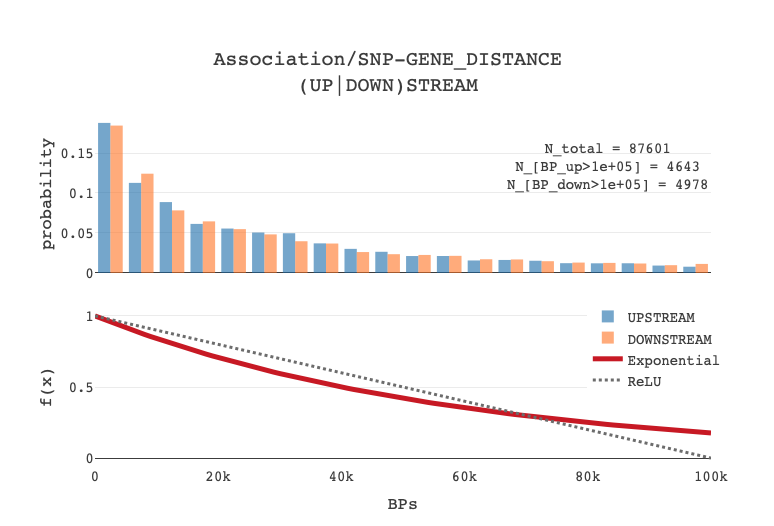
\includegraphics[width=10cm]{figures/assn_snp-gene-dist_func.png}
    \caption{SNP-gene distances and weighting function candidates}
    \label{fig:snp-gene-dist}
\end{figure}

\begin{center}
    $ W_{Exp}(d) = 2^{-d/k} $ \\
    where $ d = $ \emph{distance in base pairs} \\
    and $ k = $ \emph{"half-life distance"} (50k)
\end{center}

This function is used to weight N\_snp to compute a distance-weighted SNP count N\_snpw.

\begin{equation}
    N\_snpw = \sum_{i}^{N\_snp}  2^{-d_{i}/k}
\end{equation}

\section{Multivariate, non-parametric ranking with $\mu$ scores}

Multivariate ranking is a well studied problem which needs to be addressed for ranking GWAS associations. A weighted sum approach could be justified but requires ad hoc judgement based weights which could be fundamentally flawed and misleading. The shorthand version of the problem is how can we compare apples and oranges? In baseball, is a double worth two singles, or what is the right multiplier? From GWAS, how should effect size be weighted relative to p-value, or to the RCRAS described above? A rigorous approach exists and has been described well by Wittkowski\cite{witt_sports}, and implemented via R package muStat\cite{muStat}. Vectors of ordinal variables represent each case, and non-dominated solutions are cases which are not inferior to any other case at any variable. The set of all non-dominated solutions also define a Pareto-boundary or Pareto-front, which also is closely related to convex hull approaches. A $\mu$ score is defined simply as the number of lower cases minus the number of higher, but the ranking is the useful result. The ranking rule between case $k$ and case $k'$ may be formalized thus:

\begin{center}
$\{ x_{k} < x_{k'} \} \Leftrightarrow \{ \forall_{l=1...L}x_{kl} \leq x_{k'l} \wedge \exists_{l=1...L}x_{kl} < x_{k'l}  \}$
\end{center}


Or simply put, case k' is higher than case k if it is higher in some variable(s) and lower in none. \\
\\
Variables of merit available, for evaluating relevance and confidence of disease-gene associations, by aggregating metadata and summaries from the GWAS Catalog:

\begin{itemize}
    \item Odds ratio (OR) (median of trait-SNP ORs)
    \item pValue (median of trait-SNP pValues)
    \item N\_study (\# studies supporting association)
    \item N\_sample (median of sample sizes)
    \item 1/N\_trait (\# traits associated with this gene)
    \item 1/N\_gene (\# genes associated with this trait)
    \item N\_wsnp (\# SNPs implicating gene, weighted by distance exponential) 
    \item RCRAS (RCR aggregated score, described above)
\end{itemize}

\begin{thebibliography}{3}
\bibitem{rcr} 
BI Hutchins, X Yuan, JM Anderson, GM Santangelo. 
\textit{Relative Citation Ratio (RCR): A New Metric That Uses Citation Rates to Measure Influence at the Article Level}. 
PLoS Biol 14(9): e1002541, 2016, \texttt{https://doi.org/10.1371/journal.pbio.1002541}.

\bibitem{diseases}
Pletscher-Frankild S, Pallejà A, Tsafou K, Binder JX, Jensen LJ,
\textit{DISEASES: text mining and data integration of disease-gene associations}.
Methods. 2015 Mar;74:83-9. 
\texttt{doi:10.1016/j.ymeth.2014.11.020}.
Epub 2014 Dec 5.

\bibitem{tinx}
DC Cannon, JJ Yang, SL Mathias, O Ursu, S Mani, A Waller, SC Schürer, LJ Jensen, LA Sklar, CG Bologa, TI Oprea, Bioinformatics, 2017, btx200, 
\textit{TIN-X: Target Importance and Novelty Explorer}. 
\texttt{doi: 10.1093/bioinformatics/btx200}.

\bibitem{witt_sports}
KM Wittkowski, T Song, K Anderson, JE Daniels,
Journal of Quantitative Analysis in Sports, 4(3), 2008,
\textit{U-Scores for Multivariate Data in Sports}.
\texttt{doi:10.2202/1559-0410.1129}.

\bibitem{muStat}
Knut M. Wittkowski and Tingting Song,
\textit{muStat: Prentice Rank Sum Test and McNemar Test}, Version 1.70, Published 2012-08-23,
\texttt{https://cran.r-project.org/package=muStat}

\end{thebibliography}

\end{document}
